\documentclass[aspectratio=169,10pt]{beamer}
\usetheme{metropolis}
\usepackage{amsmath,amssymb,bm}
\usepackage{siunitx}
\usepackage{booktabs}
\usepackage[table]{xcolor}
\usepackage{tikz}
\usetikzlibrary{arrows.meta,calc,positioning,patterns}
\usepackage{pgfplots}
\pgfplotsset{compat=1.17}
\sisetup{per-mode=symbol,detect-all}
\metroset{numbering=fraction,progressbar=frametitle,block=fill}
\tikzset{capt/.style={text width=5.2cm,align=center}}
\hypersetup{colorlinks=true,urlcolor=blue!60!black,linkcolor=.}
\addtobeamertemplate{frametitle}{}{%
  \begin{tikzpicture}[remember picture,overlay]
    \node[anchor=north east,yshift=-1.5pt,xshift=-6pt] at (current page.north east) {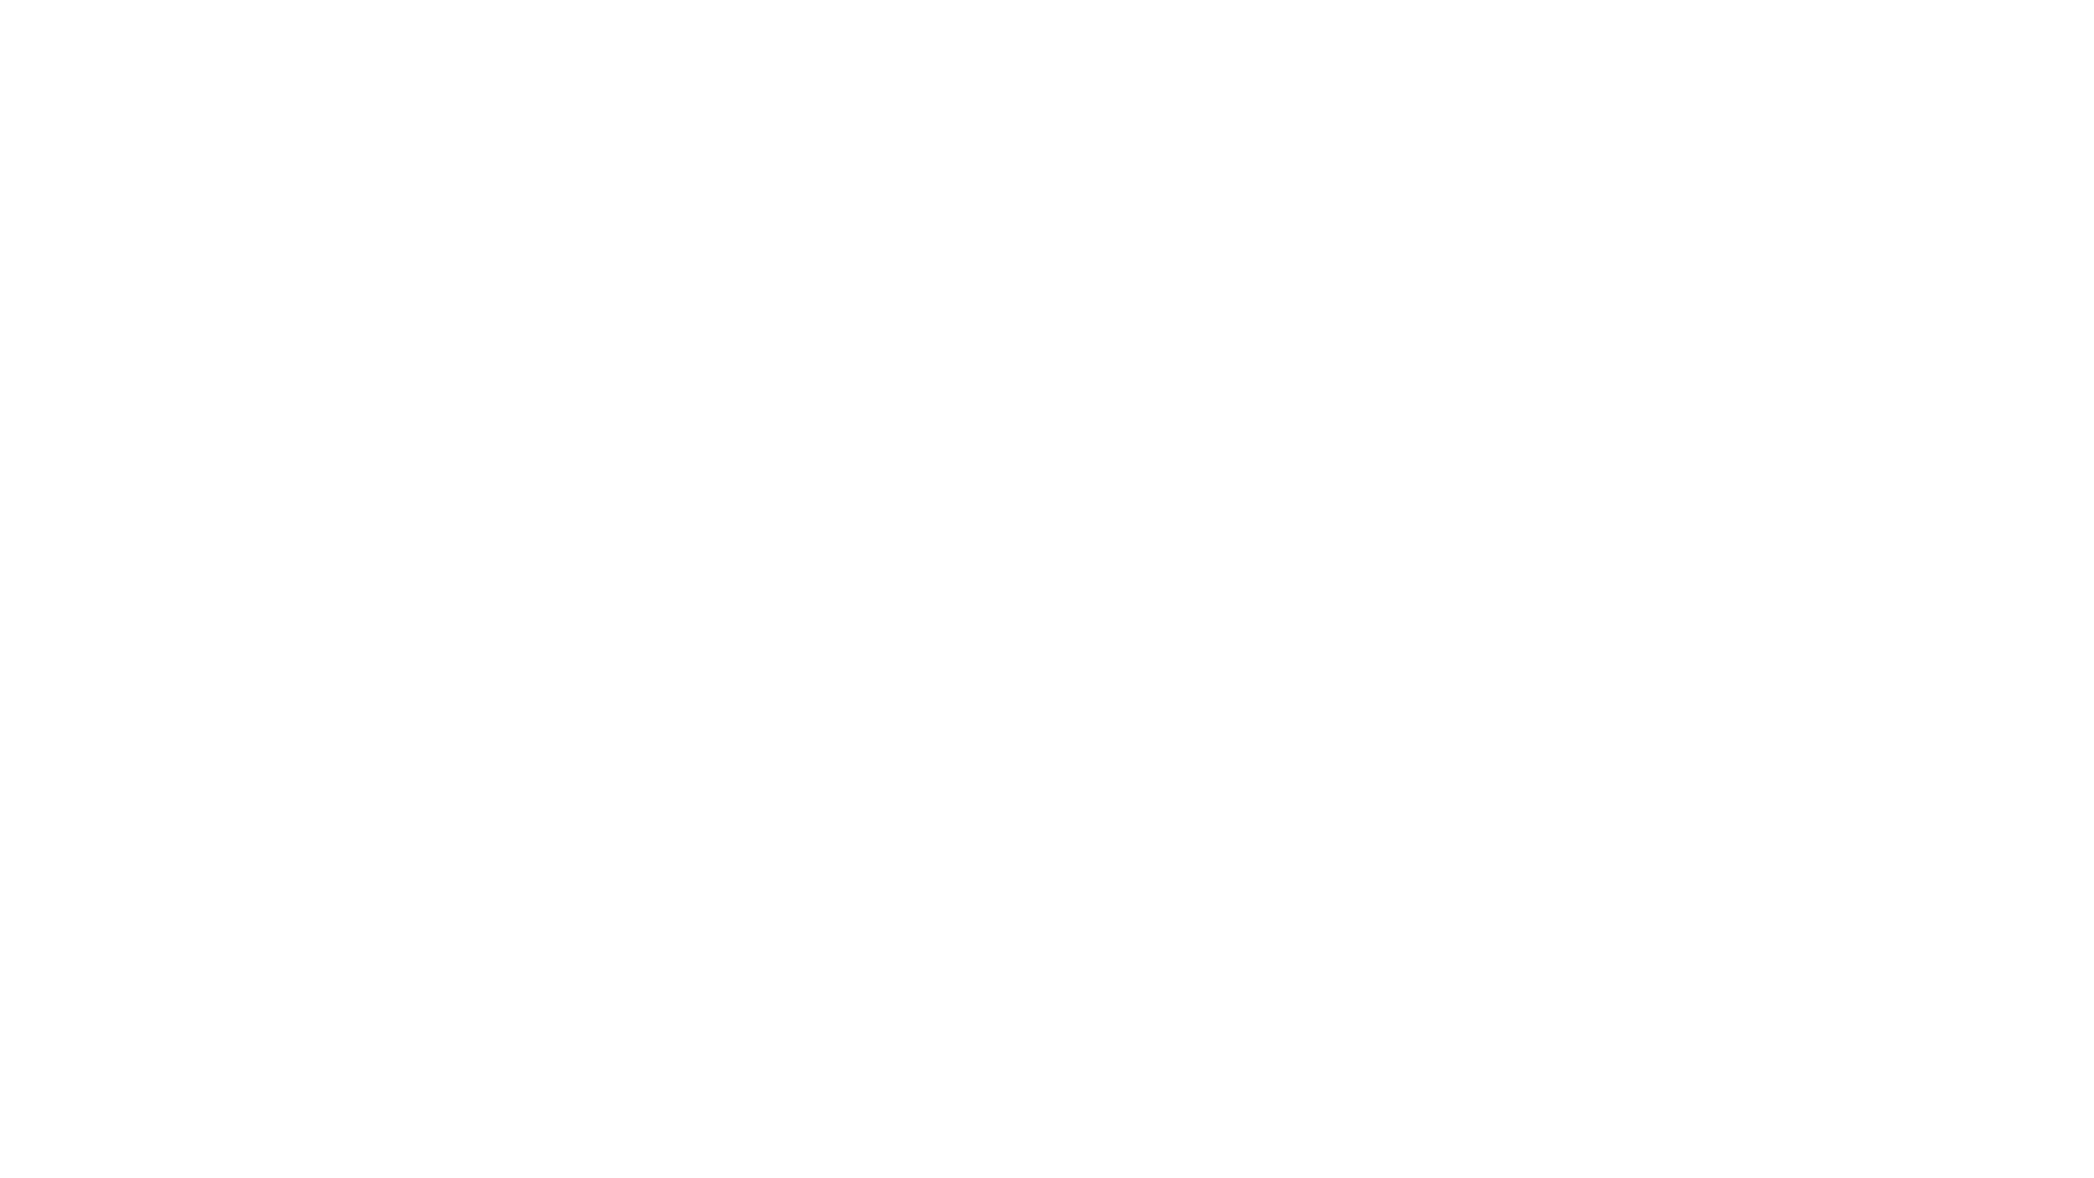
\includegraphics[height=0.7cm]{logos/itu_logo_beyaz.pdf}};
  \end{tikzpicture}}
\titlegraphic{\hfill
\includegraphics[height=1.6cm]{logos/itu_logo_laci.pdf}}

\newcommand{\wic}[1]{\raisebox{-2.6mm}{\begin{tikzpicture}[scale=0.3,line cap=round]\draw[black!35,line width=0.3pt] (-1,-1) rectangle (1,1);#1\end{tikzpicture}}}
\title{Lecture 8: Weld Groups and Adhesive Bonding}
\subtitle{Welds in bending and torsion --- UCK 364E Design of Machine Elements}
\author{Prof.\ Dr.\ Onur Tunçer}
\institute{Department of Aeronautical Engineering, Istanbul Technical University}
\date{Fall 2026}

\begin{document}
\maketitle

\begin{frame}{Today}
\begin{enumerate}
  \item When a weld carries a moment
  \item The weld as a line: unit properties
  \item Weld groups in torsion
  \item Weld groups in bending --- and where to put the weld
  \item A tube welded all round: working in N/mm
  \item Adhesive bonding: what it offers, what it asks
  \item The bonded lap: where the load actually goes
  \item Better joints, and bonding as a special process
\end{enumerate}
\end{frame}

\section{Why this lecture exists}

\begin{frame}{Last week: force over throat area. This week: a moment.}
Lecture 7: a weld carrying a force along or across its length --- divide by the throat area.

\medskip
Real welded parts are rarely that kind:
\begin{itemize}
  \item a bracket hangs a load out from a column
  \item a tube welded to a fitting is bent and twisted
\end{itemize}
\vfill
\begin{block}{You already know the method}
It is the \textbf{bolt group of Lecture 6}: a direct part, a part from the moment that grows with
distance from the centroid, added as vectors at the worst point.\\
The ``fasteners'' are now continuous, so the sums become integrals --- already done for you.
\end{block}
\end{frame}

\begin{frame}{Three ways a weld group meets a moment}
\centering
\resizebox{0.92\textwidth}{!}{% Three ways a weld group is loaded by a moment.
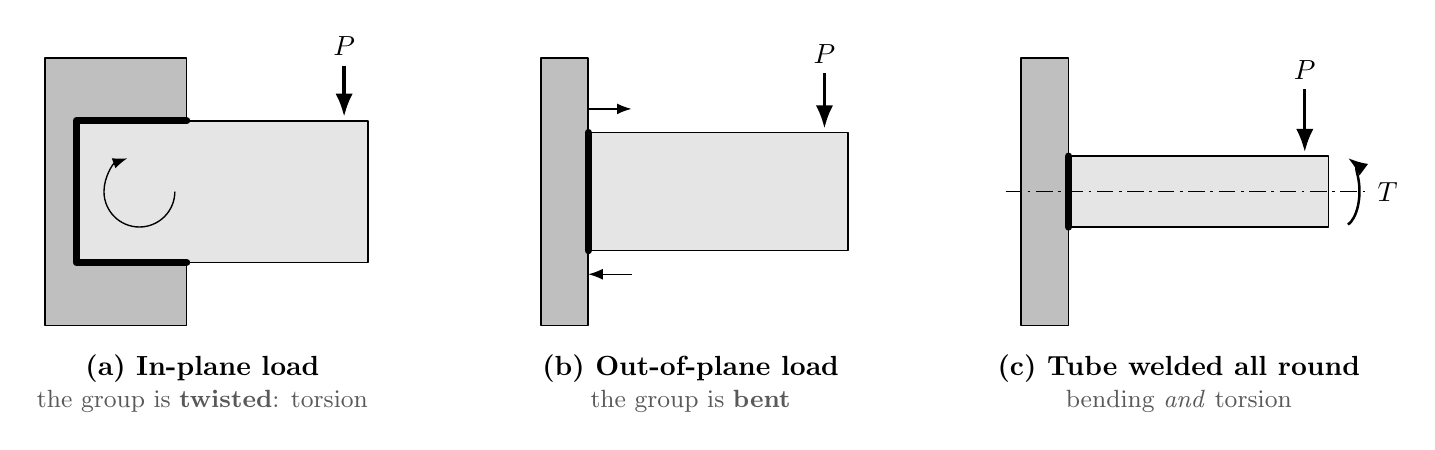
\begin{tikzpicture}[>=Latex,line join=round]
\tikzset{pl/.style={fill=black!10,draw=black,line width=0.6pt}, col/.style={fill=black!25,draw=black,line width=0.6pt},
  wd/.style={line width=2.6pt,line cap=round}, ld/.style={->,line width=1.2pt}, ttl/.style={font=\normalsize\bfseries,anchor=north,align=center},
  sub/.style={font=\small,anchor=north,align=center,text=black!65}}
% (a) in-plane: torsion
\begin{scope}
 \path[col] (-0.9,-1.7) rectangle (0.9,1.7);
 \path[pl] (-0.5,-0.9) rectangle (3.2,0.9);
 \draw[wd] (0.9,0.9) -- (-0.5,0.9) -- (-0.5,-0.9) -- (0.9,-0.9);
 \draw[ld] (2.9,1.6) -- (2.9,0.95); \node[font=\normalsize,anchor=south] at (2.9,1.6) {$P$};
 \draw[->,line width=0.5pt] (0.75,0) arc[start angle=0,end angle=-250,radius=0.45];
 \node[ttl] at (1.1,-1.95) {(a) In-plane load};
 \node[sub] at (1.1,-2.4) {the group is \textbf{twisted}: torsion};
\end{scope}
% (b) out-of-plane: bending
\begin{scope}[xshift=6.3cm]
 \path[col] (-0.9,-1.7) rectangle (-0.3,1.7);
 \path[pl] (-0.3,-0.75) rectangle (3.0,0.75);
 \draw[wd] (-0.3,0.75) -- (-0.3,-0.75);
 \draw[ld] (2.7,1.5) -- (2.7,0.8); \node[font=\normalsize,anchor=south] at (2.7,1.5) {$P$};
 \draw[->,line width=0.5pt] (-0.3,1.05) -- (0.25,1.05); \draw[->,line width=0.5pt] (0.25,-1.05) -- (-0.3,-1.05);
 \node[ttl] at (1.0,-1.95) {(b) Out-of-plane load};
 \node[sub] at (1.0,-2.4) {the group is \textbf{bent}};
\end{scope}
% (c) tube
\begin{scope}[xshift=12.4cm]
 \path[col] (-0.9,-1.7) rectangle (-0.3,1.7);
 \path[pl] (-0.3,-0.45) rectangle (3.0,0.45);
 \draw[wd] (-0.3,0.45) -- (-0.3,-0.45);
 \draw[line width=0.4pt,dash pattern=on 6pt off 2pt on 1pt off 2pt] (-1.1,0) -- (3.5,0);
 \draw[ld] (2.7,1.3) -- (2.7,0.5); \node[font=\normalsize,anchor=south] at (2.7,1.3) {$P$};
 \draw[->,line width=0.9pt] (3.25,-0.42) arc[start angle=-70,end angle=70,x radius=0.22,y radius=0.45]; \node[font=\normalsize,anchor=west] at (3.5,0) {$T$};
 \node[ttl] at (1.1,-1.95) {(c) Tube welded all round};
 \node[sub] at (1.1,-2.4) {bending \emph{and} torsion};
\end{scope}
\end{tikzpicture}
}

\medskip
\raggedright\small
(a) moment vector normal to the plane of the welds \quad (b) moment vector in that plane
\end{frame}

\section{The weld as a line}

\begin{frame}{Treat the weld as a line}
A fillet is long and thin: throat $a=0.707h$ is small beside its length.

\medskip
So every property of the group is the property of a \alert{line}, times the throat:
\[ A=a\,L,\qquad I=a\,I_u,\qquad J=a\,J_u,\qquad a=0.707\,h \]

$I_u$, $J_u$: \emph{unit} second moments about the centroid of the group, in mm$^3$.

\vfill
\begin{block}{Why this is worth doing}
Unit properties depend only on the \textbf{layout}, not on the size.\\
Choose where the weld goes first; find how big it must be second.
\end{block}
\end{frame}

\begin{frame}{Unit properties of common weld groups}
\centering\small
\renewcommand{\arraystretch}{1.45}
\begin{tabular}{@{}clll@{}}
\toprule
 & $L$ & Bending, $I_u$ (horizontal axis) & Torsion, $J_u$\\
\midrule
\wic{\draw[line width=1.6pt] (0,-1) -- (0,1);} & $d$ & $d^3/12$ & $d^3/12$\\
\wic{\draw[line width=1.6pt] (-1,-1) -- (-1,1) (1,-1) -- (1,1);} & $2d$ & $d^3/6$ & $d\,(3b^2+d^2)/6$\\
\wic{\draw[line width=1.6pt] (-1,1) -- (1,1) (-1,-1) -- (1,-1);} & $2b$ & $b\,d^2/2$ & $b\,(3d^2+b^2)/6$\\
\wic{\draw[line width=1.6pt] (1,1) -- (-1,1) -- (-1,-1) -- (1,-1);} & $2b+d$ & $d^2(6b+d)/12$ & $(8b^3+6bd^2+d^3)/12-b^4/(2b+d)$\\
\wic{\draw[line width=1.6pt] (-1,-1) rectangle (1,1);} & $2(b+d)$ & $d^2(3b+d)/6$ & $(b+d)^3/6$\\
\wic{\draw[line width=1.6pt] (0,0) circle (1);} & $2\pi r$ & $\pi r^3$ & $2\pi r^3$\\
\bottomrule
\end{tabular}

\medskip
\raggedright\footnotesize $b$ horizontal, $d$ vertical. Three-sided: centroid $\bar x=b^2/(2b+d)$ from
the closed side. \ Check: $J_u=I_{u,x}+I_{u,y}$. \ (Shigley Tables 9--1, 9--2)
\end{frame}

\section{Weld groups in torsion}

\begin{frame}{Torsion: the load is in the plane of the welds}
Move the load to the centroid: a force $V$ and a moment $M=Ve$.

\begin{enumerate}
\item \textbf{Primary shear} --- the same everywhere, along the load:
  \[ \tau'=\frac{V}{A} \]
\item \textbf{Secondary shear} --- perpendicular to the radius, proportional to it:
  \[ \tau''=\frac{M\,r}{J} \]
\item \textbf{Add as vectors} at the worst point: furthest from the centroid, on the side nearest the load.
\end{enumerate}
\vfill
Lecture 6 word for word, with $A$ in place of $n$ and $J$ in place of $\sum r^2$.
\end{frame}

\begin{frame}{Example 8.1 --- a bracket welded on three sides}
\begin{columns}[c]
\begin{column}{0.52\textwidth}
\resizebox{\textwidth}{!}{% Example 8.1: a C-shaped weld group in torsion. 1 mm = 0.035 cm.
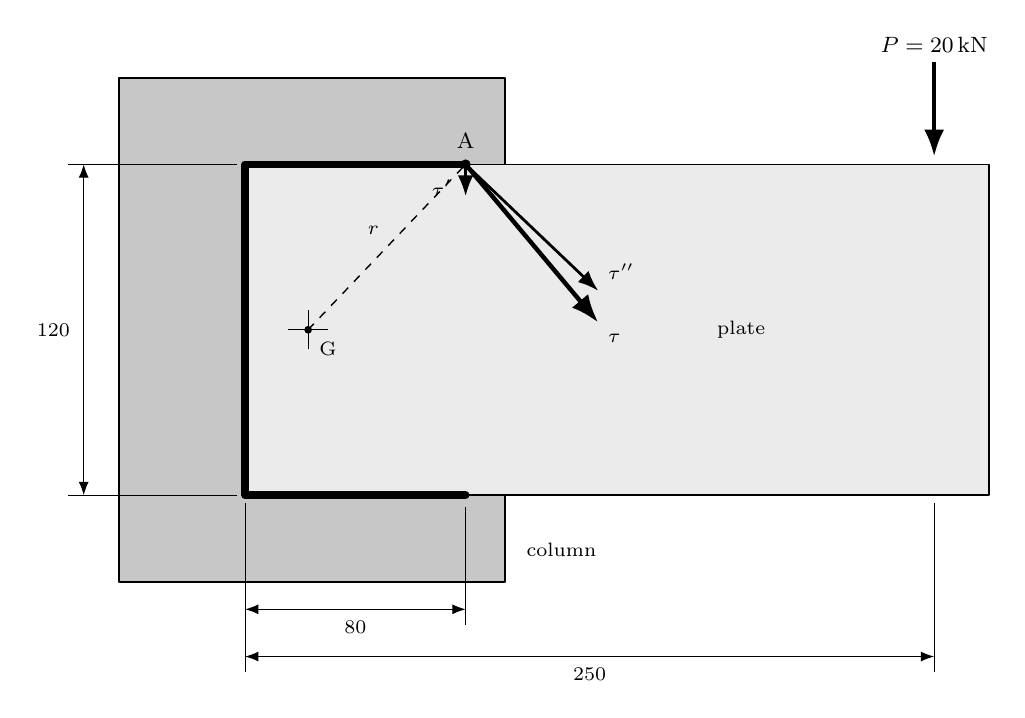
\begin{tikzpicture}[>=Latex,line join=round]
\tikzset{lb/.style={font=\footnotesize}, sm/.style={font=\scriptsize}, dimn/.style={<->,line width=0.4pt}, ext/.style={line width=0.25pt}}
\def\g{0.035}
\fill[black!22] (-1.6,-3.2) rectangle (3.3,3.2); \draw[line width=0.6pt] (-1.6,-3.2) rectangle (3.3,3.2);
\fill[black!8] (0,-60*\g) rectangle (270*\g,60*\g); \draw[line width=0.6pt] (0,-60*\g) rectangle (270*\g,60*\g);
\draw[line width=2.8pt,line cap=round] (80*\g,60*\g) -- (0,60*\g) -- (0,-60*\g) -- (80*\g,-60*\g);
% centroid
\def\xb{22.86}
\draw[line width=0.3pt] (\xb*\g-0.25,0) -- (\xb*\g+0.25,0) (\xb*\g,-0.25) -- (\xb*\g,0.25); \fill (\xb*\g,0) circle (1.4pt);
\node[sm,anchor=north west] at (\xb*\g+0.02,-0.04) {G};
% load
\draw[->,line width=1.5pt] (250*\g,3.4) -- (250*\g,2.2); \node[lb,anchor=south] at (250*\g,3.4) {$P=\SI{20}{kN}$};
% radius to A
\draw[line width=0.5pt,dashed] (\xb*\g,0) -- (80*\g,60*\g); \node[sm,anchor=south east] at (52*\g,31*\g) {$r$};
\fill (80*\g,60*\g) circle (1.8pt); \node[lb,anchor=south] at (80*\g,60*\g+0.08) {A};
% vectors at A : tau' down, tau'' perpendicular to r (clockwise): direction (y,-x)/r = (60,-57.14)/82.86
\def\f{0.024}
\draw[->,line width=1.0pt] (80*\g,60*\g) -- ++(0,-16.84*\f);
\draw[->,line width=1.0pt] (80*\g,60*\g) -- ++(70.2*\f,-66.9*\f);
\draw[->,line width=1.6pt] (80*\g,60*\g) -- ++(70.2*\f,-83.7*\f);
\node[sm,anchor=east] at (80*\g-0.05,60*\g-0.3) {$\tau'$};
\node[sm,anchor=south west] at (80*\g+70.2*\f,60*\g-66.9*\f+0.02) {$\tau''$};
\node[sm,anchor=north west] at (80*\g+70.2*\f,60*\g-83.7*\f-0.02) {$\tau$};
% dimensions
\draw[ext] (0,-60*\g-0.1) -- (0,-3.75) (80*\g,-60*\g-0.15) -- (80*\g,-3.75) (250*\g,-60*\g-0.1) -- (250*\g,-4.35) (0,-3.75) -- (0,-4.35);
\draw[dimn] (0,-3.55) -- (80*\g,-3.55); \node[sm,anchor=north] at (40*\g,-3.57) {80};
\draw[dimn] (0,-4.15) -- (250*\g,-4.15); \node[sm,anchor=north] at (125*\g,-4.17) {250};
\draw[ext] (-0.1,60*\g) -- (-2.25,60*\g) (-0.1,-60*\g) -- (-2.25,-60*\g); \draw[dimn] (-2.05,-60*\g) -- (-2.05,60*\g); \node[sm,anchor=east] at (-2.1,0) {120};
\node[sm,anchor=west] at (3.45,-2.8) {column};
\node[sm] at (6.3,0) {plate};
\end{tikzpicture}
}
\end{column}
\begin{column}{0.46\textwidth}
\small
$h=\SI{6}{mm}$, $b=80$, $d=\SI{120}{mm}$\\
$P=\SI{20}{kN}$ at \SI{250}{mm} from the vertical run\\
E70xx: $\tau_{\text{all}}=\SI{145}{MPa}$

\medskip
\textbf{Group}\\
$L=\SI{280}{mm}$, \ $A=\SI{1188}{mm^2}$\\
$\bar x=80^2/280=\SI{22.9}{mm}$\\
$J_u=\SI{915000}{mm^3}$\\
$J=0.707(6)J_u=\SI{3.88e6}{mm^4}$

\medskip
\textbf{At the centroid}\\
$e=250-22.9=\SI{227.1}{mm}$\\
$M=\SI{4.54e6}{N.mm}$
\end{column}
\end{columns}
\end{frame}

\begin{frame}{Example 8.1 --- the critical point}
Point A, tip of the upper run: $x=\SI{57.1}{mm}$, $y=\SI{60}{mm}$, $r=\SI{82.9}{mm}$
\[ \tau'=\frac{20\,000}{1188}=\SI{16.8}{MPa}\ \text{(down)} \]
\[ \tau''_x=\frac{M\,y}{J}=\SI{70.2}{MPa},\qquad \tau''_y=\frac{M\,x}{J}=\SI{66.9}{MPa}\ \text{(down)} \]
\[ \tau=\sqrt{70.2^2+(66.9+16.8)^2}=\alert{\SI{109}{MPa}}\qquad n=145/109=1.33 \]
\vfill
\begin{alertblock}{Read the numbers}
Moment: \SI{97}{MPa}. Direct shear: \SI{17}{MPa}.\\
Load over throat area would have reported \SI{17}{MPa} and a factor of 8.6.
\end{alertblock}
\end{frame}

\section{Weld groups in bending}

\begin{frame}{Bending: the load is out of the plane of the welds}
The moment pulls one edge of the group off and pushes the other on.
\[ \tau'=\frac{V}{A},\qquad \tau''=\frac{M\,c}{I},\qquad \tau=\sqrt{\tau'^2+\tau''^2} \]

Two conventions, both from Lecture 7:
\begin{itemize}
  \item the bending stress is normal to the weld line, but is \alert{treated as a shear on the throat}
  \item direct shear and bending stress are at right angles: root of the sum of squares
\end{itemize}
\vfill
$I=0.707\,h\,I_u$, with $I_u$ about the neutral axis of the group.
\end{frame}

\begin{frame}{Example 8.2 --- three ways to weld the same bracket}
\centering
\resizebox{0.95\textwidth}{!}{% Example 8.2: the same weld length arranged three ways, seen looking along the bracket.
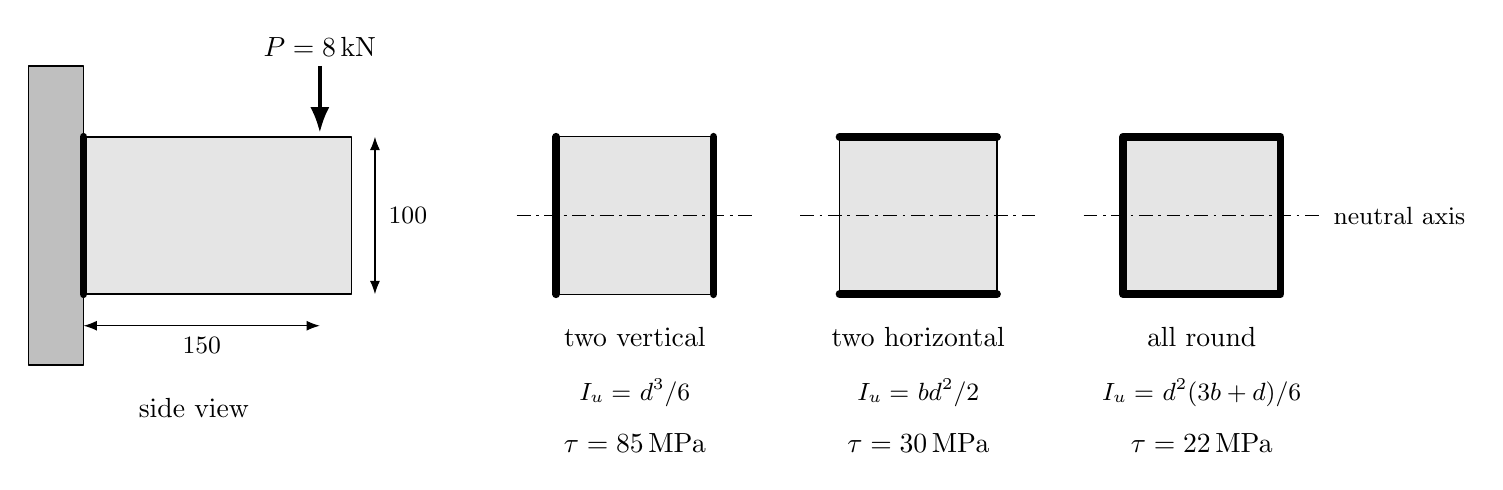
\begin{tikzpicture}[>=Latex,line join=round]
\tikzset{lb/.style={font=\normalsize}, sm/.style={font=\small}, wd/.style={line width=2.8pt,line cap=round}, sec/.style={fill=black!10,draw=black,line width=0.5pt}}
% side view
\begin{scope}
 \fill[black!25] (-0.7,-1.9) rectangle (0,1.9); \draw[line width=0.6pt] (-0.7,-1.9) rectangle (0,1.9);
 \fill[black!10] (0,-1.0) rectangle (3.4,1.0); \draw[line width=0.6pt] (0,-1.0) rectangle (3.4,1.0);
 \draw[wd] (0,1.0) -- (0,-1.0);
 \draw[->,line width=1.4pt] (3.0,1.9) -- (3.0,1.05); \node[lb,anchor=south] at (3.0,1.9) {$P=\SI{8}{kN}$};
 \draw[<->,line width=0.4pt] (0,-1.4) -- (3.0,-1.4); \node[sm,anchor=north] at (1.5,-1.42) {150};
 \draw[<->,line width=0.4pt] (3.7,-1.0) -- (3.7,1.0); \node[sm,anchor=west] at (3.75,0) {100};
 \node[lb,anchor=north] at (1.4,-2.2) {side view};
\end{scope}
% three weld patterns, end view
\foreach \xo/\ttl/\iu/\tv in {7.0/{two vertical}/{$d^3/6$}/85, 10.6/{two horizontal}/{$bd^2/2$}/30, 14.2/{all round}/{$d^2(3b+d)/6$}/22}{
 \begin{scope}[xshift=\xo cm]
  \path[sec] (-1.0,-1.0) rectangle (1.0,1.0);
  \draw[line width=0.3pt,dash pattern=on 5pt off 2pt on 1pt off 2pt] (-1.5,0) -- (1.5,0);
  \node[lb,anchor=north] at (0,-1.3) {\ttl};
  \node[sm,anchor=north] at (0,-1.95) {$I_u=$ \iu};
  \node[lb,anchor=north] at (0,-2.65) {$\tau=\SI{\tv}{MPa}$};
 \end{scope}}
\begin{scope}[xshift=7.0cm] \draw[wd] (-1.0,-1.0) -- (-1.0,1.0) (1.0,-1.0) -- (1.0,1.0); \end{scope}
\begin{scope}[xshift=10.6cm] \draw[wd] (-1.0,1.0) -- (1.0,1.0) (-1.0,-1.0) -- (1.0,-1.0); \end{scope}
\begin{scope}[xshift=14.2cm] \draw[wd] (-1.0,-1.0) rectangle (1.0,1.0); \end{scope}
\node[sm,anchor=west] at (15.75,0) {neutral axis};
\end{tikzpicture}
}

\medskip
\small $P=\SI{8}{kN}$ at \SI{150}{mm}; \ $M=\SI{1.2e6}{N.mm}$; \ $h=\SI{6}{mm}$; \ $c=\SI{50}{mm}$
\end{frame}

\begin{frame}{Example 8.2 --- the numbers}
\centering
\renewcommand{\arraystretch}{1.3}
\begin{tabular}{@{}lccccc@{}}
\toprule
Arrangement & Weld, mm & $I_u$, mm$^3$ & $\tau'$ & $\tau''$ & $\tau$, MPa\\
\midrule
(a) two vertical & 200 & 166\,700 & 9.4 & 84.9 & \textbf{85}\\
(b) two horizontal & 200 & 500\,000 & 9.4 & 28.3 & \textbf{30}\\
(c) all round & 400 & 666\,700 & 4.7 & 21.2 & \textbf{22}\\
\bottomrule
\end{tabular}

\vfill
\raggedright
Same weld, moved from the sides to the top and bottom: stress down by \alert{2.9}.\\
Doubling the weld after that: another 1.4.

\medskip
\begin{block}{Weld metal far from the neutral axis does the work}
Exactly as flange material does in a beam.
\end{block}
\end{frame}

\begin{frame}{The catch}
Arrangement (b) puts a \textbf{transverse weld across the most highly stressed fibre} of the bracket.

\medskip
\begin{itemize}
  \item Statically: the right answer.
  \item If the load cycles: that weld toe is where the crack starts.
\end{itemize}
\vfill
\begin{alertblock}{Static strength and fatigue pull in opposite directions}
Put the weld where the lever arm is --- then check the toe there as a fatigue detail (Lecture 7).
\end{alertblock}
\end{frame}

\section{A tube welded all round}

\begin{frame}{For sizing, work in force per unit length}
You do not know the weld size yet. Divide the loads by the \emph{line} properties: $f$ in N/mm.
\[ a=\frac{f}{\tau_{\text{all}}},\qquad h=\frac{a}{0.707} \]
Ring of weld, radius $r$: \ $L=2\pi r$, \ $I_u=\pi r^3$, \ $J_u=2\pi r^3$
\[ f_N=\frac{N}{2\pi r},\qquad f_M=\frac{M}{\pi r^2},\qquad f_T=\frac{T}{2\pi r^2} \]
\vfill
$f_N$ and $f_M$ act along the tube axis and add directly at the extreme fibre.\\
$f_T$ acts around the circumference, at right angles to them.
\end{frame}

\begin{frame}{Example 8.3 --- the end weld of an engine-mount tube}
\footnotesize
$25.4\times\SI{0.889}{mm}$ 4130N tube, fillet all round. Limit: $N=\SI{12}{kN}$, $M=\SI{40}{N.m}$,
$T=\SI{30}{N.m}$. Weld metal $F_{su}=\SI{300}{MPa}$.
\[ f_N=\SI{150}{N/mm},\qquad f_M=\SI{79}{N/mm},\qquad f_T=\SI{30}{N/mm} \]
\[ f=\sqrt{(150+79)^2+30^2}=\SI{231}{N/mm}\ \text{limit}\quad\Rightarrow\quad f_u=1.5\times231=\SI{347}{N/mm} \]
\[ a=\frac{347}{300}=\SI{1.16}{mm},\qquad h=\alert{\SI{1.6}{mm}}\quad\text{--- call up a1.2 all round} \]

\textbf{The tube beside the weld:} $A=\SI{68.5}{mm^2}$, $Z=\SI{419}{mm^3}$
\[ \sigma=175+95=\SI{271}{MPa}\ \text{limit},\ \SI{406}{MPa}\ \text{ultimate};\qquad \mathrm{MS}=\frac{552}{406}-1=\alert{+0.36} \]

Two margins, two materials. \textbf{Project 1 needs both at every cluster.}
\end{frame}

\begin{frame}{If the load cycles}
Nothing here changes the fatigue rules of Lecture 7. It tells you \alert{where} to apply them.

\medskip
\begin{itemize}
  \item Find the stress \emph{range} at the critical point of the group
  \item Load-carrying fillet: check the root, on the throat stress
  \item Member beside it: check the toe, with the detail category that fits
\end{itemize}
\vfill
Shigley's worst factor was the \textbf{end of a parallel fillet}.\\
In Example 8.1 that is exactly point A.
\end{frame}

\section{Adhesive bonding}

\begin{frame}{The last permanent joint: no fastener and no heat}
\begin{columns}[T]
\begin{column}{0.48\textwidth}
\textbf{In its favour}
\begin{itemize}
  \item no holes: no net-section loss
  \item load spread over an area
  \item seals the joint
  \item joins thin sheet and dissimilar materials
  \item fatigue life far better than a riveted joint
\end{itemize}
\end{column}
\begin{column}{0.48\textwidth}
\textbf{Against it}
\begin{itemize}
  \item strength depends on a surface preparation you cannot see afterwards
  \item weak in peel
  \item moisture, temperature, creep
  \item cannot be taken apart
  \item \alert{no inspection measures the strength of a finished bond}
\end{itemize}
\end{column}
\end{columns}
\end{frame}

\begin{frame}{Where you meet it}
\begin{itemize}
  \item \textbf{Honeycomb sandwich} --- floors, control surfaces, fairings: face sheets held to the
        core by adhesive and nothing else
  \item \textbf{Bonded stringers} --- de Havilland in wood in the 1940s, the Fokker F27 in metal in the 1950s
  \item \textbf{Every composite structure}
  \item \textbf{Threadlocker} (Lecture 5) --- an anaerobic adhesive, cured by shutting out the air
\end{itemize}
\end{frame}

\begin{frame}{Four ways to load an adhesive}
\centering
\resizebox{0.95\textwidth}{!}{% The four ways to load an adhesive joint.
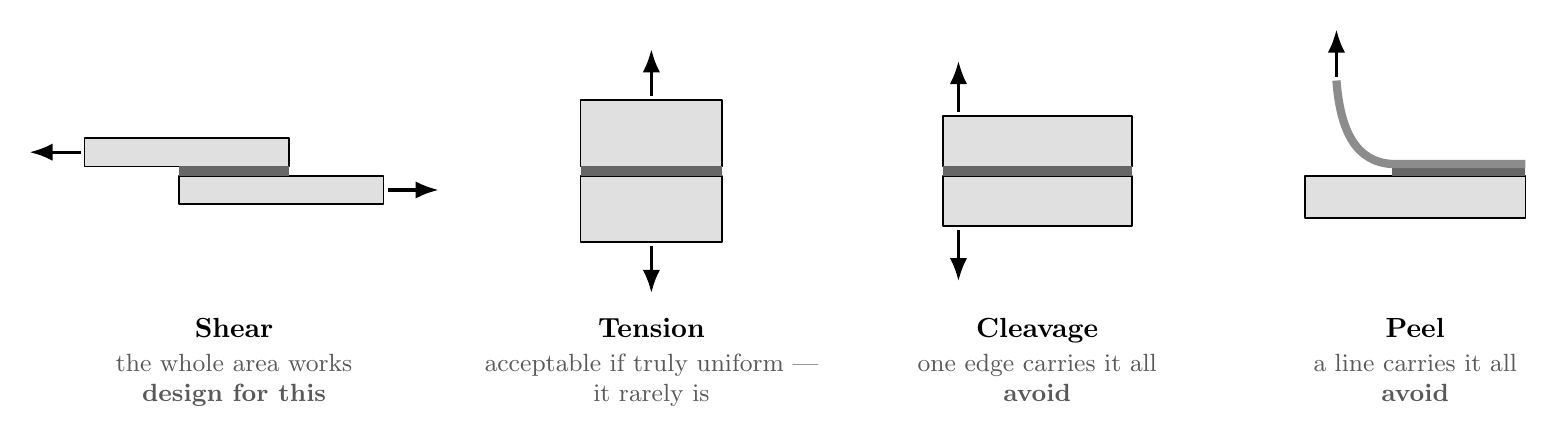
\begin{tikzpicture}[>=Latex,line join=round]
\tikzset{ad/.style={fill=black!12,draw=black,line width=0.6pt}, gl/.style={fill=black!60}, ld/.style={->,line width=1.2pt},
  ttl/.style={font=\normalsize\bfseries,anchor=north}, sub/.style={font=\small,anchor=north,text=black!65,align=center}}
% shear
\begin{scope}
 \path[ad] (-1.9,0.06) rectangle (0.7,0.42); \path[ad] (-0.7,-0.42) rectangle (1.9,-0.06); \path[gl] (-0.7,-0.06) rectangle (0.7,0.06);
 \draw[ld] (-1.95,0.24) -- (-2.6,0.24); \draw[ld] (1.95,-0.24) -- (2.6,-0.24);
 \node[ttl] at (0,-1.75) {Shear}; \node[sub] at (0,-2.2) {the whole area works\\ \textbf{design for this}};
\end{scope}
% tension
\begin{scope}[xshift=5.3cm]
 \path[ad] (-0.9,0.06) rectangle (0.9,0.9); \path[ad] (-0.9,-0.9) rectangle (0.9,-0.06); \path[gl] (-0.9,-0.06) rectangle (0.9,0.06);
 \draw[ld] (0,0.95) -- (0,1.55); \draw[ld] (0,-0.95) -- (0,-1.55);
 \node[ttl] at (0,-1.75) {Tension}; \node[sub] at (0,-2.2) {acceptable if truly uniform ---\\ it rarely is};
\end{scope}
% cleavage
\begin{scope}[xshift=10.2cm]
 \path[ad] (-1.2,0.06) rectangle (1.2,0.7); \path[ad] (-1.2,-0.7) rectangle (1.2,-0.06); \path[gl] (-1.2,-0.06) rectangle (1.2,0.06);
 \draw[ld] (-1.0,0.75) -- (-1.0,1.4); \draw[ld] (-1.0,-0.75) -- (-1.0,-1.4);
 \node[ttl] at (0,-1.75) {Cleavage}; \node[sub] at (0,-2.2) {one edge carries it all\\ \textbf{avoid}};
\end{scope}
% peel
\begin{scope}[xshift=15.0cm]
 \path[ad] (-1.4,-0.6) rectangle (1.4,-0.06); \path[gl] (-0.3,-0.06) rectangle (1.4,0.04);
 \draw[line width=3pt,black!45,line cap=butt] (1.4,0.09) -- (-0.3,0.09) .. controls (-0.75,0.12) and (-0.95,0.5) .. (-1.0,1.15);
 \draw[ld] (-1.0,1.2) -- (-1.0,1.8);
 \node[ttl] at (0,-1.75) {Peel}; \node[sub] at (0,-2.2) {a line carries it all\\ \textbf{avoid}};
\end{scope}
\end{tikzpicture}
}

\vfill
\begin{block}{The whole art of bonded joint design}
Arrange the joint so the adhesive is in \textbf{shear}. Keep peel and cleavage out.
\end{block}
\end{frame}

\begin{frame}{Adhesive families}
\centering\small
\begin{tabular}{@{}llll@{}}
\toprule
Family & Lap shear, MPa & Service limit & Where\\
\midrule
Epoxy film, hot cured & 25--40 & 120--\SI{175}{\degree C} & primary structure, honeycomb\\
Epoxy paste, two-part & 15--30 & $\sim$\SI{80}{\degree C} & repairs, fittings, shimming\\
Toughened acrylic & 15--25 & $\sim$\SI{100}{\degree C} & fast assembly\\
Anaerobic & 10--25 & $\sim$\SI{150}{\degree C} & threadlocking, retaining\\
Cyanoacrylate & 10--20 & $\sim$\SI{80}{\degree C} & small parts; brittle\\
Polyurethane, silicone & 1--15 & to \SI{200}{\degree C} & sealing, flexible joints\\
\bottomrule
\end{tabular}

\vfill
\raggedright
Indicative room-temperature figures. Design with the data sheet value for \emph{your} adherends,
preparation and temperature --- far lower \textbf{hot and wet}.
\end{frame}

\begin{frame}{The lap joint: the obvious calculation is misleading}
\[ \tau_{\text{avg}}=\frac{P}{b\,l} \]
As misleading as dividing a row of fasteners equally --- and for the same reason.

\medskip
\begin{itemize}
  \item At one end, one sheet carries all the load and the other none: they stretch differently,
        and the adhesive between them is sheared hard.
  \item In the middle both carry half and stretch alike: the adhesive has almost nothing to do.
\end{itemize}
\end{frame}

\begin{frame}{Shear lag (Volkersen)}
Identical sheets $t$, $E$; adhesive layer $t_a$, shear modulus $G$:
\[ \frac{\tau_{\max}}{\tau_{\text{avg}}}=\frac{\omega l}{2}\,\coth\frac{\omega l}{2},\qquad \omega=\sqrt{\frac{2G}{E\,t\,t_a}} \]
For a long overlap $\coth\to1$:
\[ \tau_{\max}\approx\frac{P\,\omega}{2b} \]
\vfill
\begin{alertblock}{The overlap length has cancelled}
Beyond a certain length, more overlap does nothing for the peak stress.
\end{alertblock}
\end{frame}

\begin{frame}{Example 8.4 --- same load, three overlaps}
\centering
\resizebox{!}{0.8\textheight}{% Shear stress along a bonded single lap for three overlaps, same load. Example 8.4.
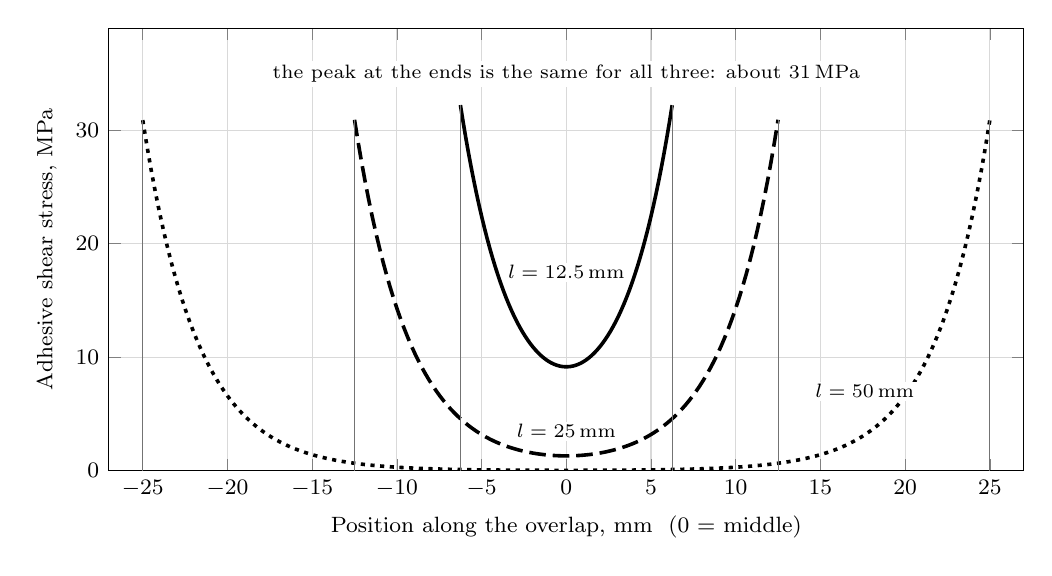
\begin{tikzpicture}
\begin{axis}[width=13.2cm,height=7.2cm,xmin=-27,xmax=27,ymin=0,ymax=39,
  xlabel={Position along the overlap, mm \ (0 = middle)},ylabel={Adhesive shear stress, MPa},
  label style={font=\footnotesize},tick label style={font=\footnotesize},grid=major,major grid style={black!15},clip=true]
% tau(x) = (P w / (2 b)) cosh(w x)/sinh(w l/2),  P=5000 N, b=25 mm, w=0.3090 /mm
\addplot[black,line width=1.3pt,domain=-6.25:6.25,samples=80] {30.90*cosh(0.3090*x)/sinh(0.3090*6.25)};
\addplot[black,line width=1.3pt,dash pattern=on 6pt off 2.5pt,domain=-12.5:12.5,samples=120] {30.90*cosh(0.3090*x)/sinh(0.3090*12.5)};
\addplot[black,line width=1.3pt,dash pattern=on 1.5pt off 2pt,domain=-25:25,samples=200] {30.90*cosh(0.3090*x)/sinh(0.3090*25)};
\addplot[black!55,line width=0.4pt] coordinates {(-6.25,0) (-6.25,32.2)}; \addplot[black!55,line width=0.4pt] coordinates {(6.25,0) (6.25,32.2)};
\addplot[black!55,line width=0.4pt] coordinates {(-12.5,0) (-12.5,30.9)}; \addplot[black!55,line width=0.4pt] coordinates {(12.5,0) (12.5,30.9)};
\addplot[black!55,line width=0.4pt] coordinates {(-25,0) (-25,30.9)}; \addplot[black!55,line width=0.4pt] coordinates {(25,0) (25,30.9)};
\node[font=\scriptsize,anchor=south,fill=white,inner sep=1pt] at (axis cs:0,16.6) {$l=\SI{12.5}{mm}$};
\node[font=\scriptsize,anchor=south,fill=white,inner sep=1pt] at (axis cs:0,2.6) {$l=\SI{25}{mm}$};
\node[font=\scriptsize,anchor=west,fill=white,inner sep=1pt] at (axis cs:14.5,7) {$l=\SI{50}{mm}$};
\node[font=\scriptsize,anchor=south,fill=white,inner sep=1.5pt] at (axis cs:0,33.8) {the peak at the ends is the same for all three: about \SI{31}{MPa}};
\end{axis}
\end{tikzpicture}
}
\end{frame}

\begin{frame}{Example 8.4 --- a longer overlap is not a stronger joint}
\small 2024-T3, $t=\SI{1.6}{mm}$, $b=\SI{25}{mm}$; epoxy $G=\SI{1.1}{GPa}$, $t_a=\SI{0.2}{mm}$; $P=\SI{5}{kN}$; \ $\omega=\SI{0.309}{mm^{-1}}$

\medskip
\centering\normalsize
\begin{tabular}{@{}ccccc@{}}
\toprule
$l$, mm & $\tau_{\text{avg}}$, MPa & $\omega l/2$ & $\tau_{\max}/\tau_{\text{avg}}$ & $\tau_{\max}$, MPa\\
\midrule
12.5 & 16.0 & 1.93 & 2.01 & 32.2\\
25 & 8.0 & 3.86 & 3.87 & 30.9\\
50 & 4.0 & 7.73 & 7.73 & 30.9\\
\bottomrule
\end{tabular}

\vfill
\raggedright
Four times the overlap, four times the adhesive: the peak falls by \alert{four per cent}.

\medskip
What does lower the peak: \textbf{thicker or stiffer adherends}, a \textbf{thicker bond line}, a
\textbf{more flexible adhesive}.
\end{frame}

\begin{frame}{Two cautions}
\begin{enumerate}
  \item \textbf{The analysis is elastic.} A real adhesive yields at the ends before it breaks; the
        joint is stronger than the elastic number says. The conclusion about overlap survives.\\[3pt]
        The lightly stressed middle is not wasted: it resists creep. Rule of thumb for thin
        aluminium: overlap of roughly 20 to 30 sheet thicknesses.
  \item \textbf{Shear lag leaves out the worst part.} A single lap is eccentric, so it bends ---
        and the bending \alert{peels} the ends apart.
\end{enumerate}
\end{frame}

\begin{frame}{Better joints}
\centering
\resizebox{!}{0.72\textheight}{% Bonded joint configurations, from worst to best.
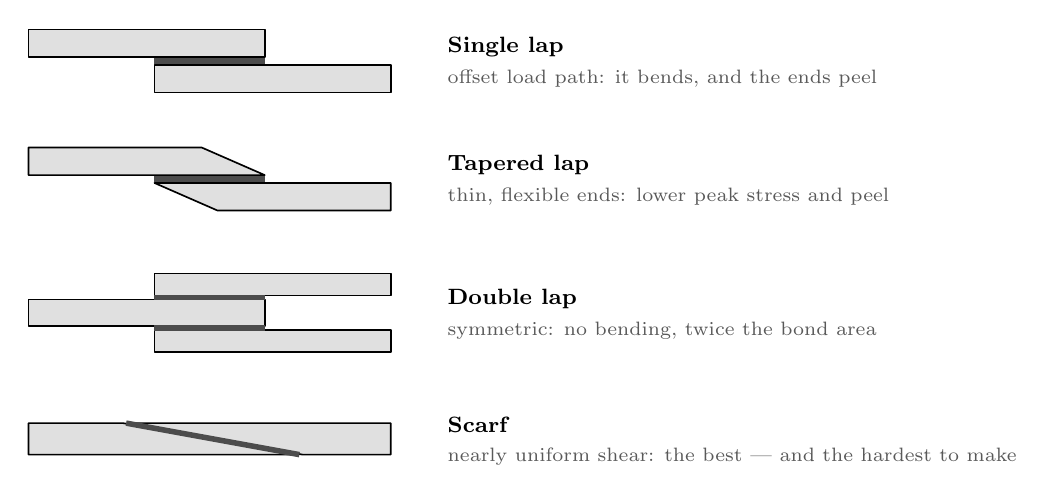
\begin{tikzpicture}[line join=round,>=Latex]
\tikzset{ad/.style={fill=black!12,draw=black,line width=0.6pt}, gl/.style={black!70,line width=2pt,line cap=butt},
  ttl/.style={font=\footnotesize\bfseries,anchor=west}, sub/.style={font=\scriptsize,anchor=west,text=black!65}}
% single lap
\begin{scope}
 \path[ad] (0,0.05) rectangle (3.0,0.4); \path[ad] (1.6,-0.4) rectangle (4.6,-0.05); \draw[gl] (1.6,0) -- (3.0,0);
 \node[ttl] at (5.2,0.18) {Single lap}; \node[sub] at (5.2,-0.22) {offset load path: it bends, and the ends peel};
\end{scope}
\begin{scope}[yshift=-1.5cm]
 \path[ad] (0,0.05) -- (2.2,0.05) -- (3.0,0.05) -- (2.2,0.4) -- (0,0.4) -- cycle; \path[ad] (1.6,-0.05) -- (2.4,-0.4) -- (4.6,-0.4) -- (4.6,-0.05) -- cycle; \draw[gl] (1.6,0) -- (3.0,0);
 \node[ttl] at (5.2,0.18) {Tapered lap}; \node[sub] at (5.2,-0.22) {thin, flexible ends: lower peak stress and peel};
\end{scope}
\begin{scope}[yshift=-3.2cm]
 \path[ad] (0,-0.17) rectangle (3.0,0.17); \path[ad] (1.6,0.22) rectangle (4.6,0.5); \path[ad] (1.6,-0.5) rectangle (4.6,-0.22); \draw[gl] (1.6,0.195) -- (3.0,0.195) (1.6,-0.195) -- (3.0,-0.195);
 \node[ttl] at (5.2,0.18) {Double lap}; \node[sub] at (5.2,-0.22) {symmetric: no bending, twice the bond area};
\end{scope}
\begin{scope}[yshift=-4.8cm]
 \path[ad] (0,-0.2) -- (3.4,-0.2) -- (1.2,0.2) -- (0,0.2) -- cycle; \path[ad] (3.48,-0.2) -- (4.6,-0.2) -- (4.6,0.2) -- (1.28,0.2) -- cycle; \draw[gl] (3.44,-0.2) -- (1.24,0.2);
 \node[ttl] at (5.2,0.18) {Scarf}; \node[sub] at (5.2,-0.22) {nearly uniform shear: the best --- and the hardest to make};
\end{scope}
\end{tikzpicture}
}

\medskip
\small Each step removes some of the bending, the peel, or the stiffness jump at the ends.
\end{frame}

\begin{frame}{One idea, met three times}
\begin{block}{A joint transfers load at its ends}
Where the two parts are trying to stretch by different amounts.
\end{block}
\begin{itemize}
  \item Fasteners in a row (Lecture 6): the end fasteners carry most
  \item A long parallel fillet (Lecture 7): the ends carry most
  \item A bonded overlap: the ends carry nearly all
\end{itemize}
\vfill
Adding length adds material where nothing is happening.

\medskip
The cure is always the same: make the stiffness change \alert{gradually} --- taper the splice
plate, taper the adherend, scarf the joint.
\end{frame}

\begin{frame}{Bonding is a special process --- more so than welding}
The bond is made at an oxide layer a few tens of nanometres thick.\\
Whether the adhesive gripped it cannot be seen or measured afterwards.

\medskip
So the quality is controlled before and during:
\begin{itemize}
  \item qualified surface treatment --- for aluminium, anodise and primer
  \item a time limit between preparation and bonding
  \item controlled cure temperature and pressure
  \item controlled bond-line thickness
  \item test coupons made with every batch, and broken
\end{itemize}
\end{frame}

\begin{frame}{Aloha 243, read again as a bonding failure}
Early 737 fuselage lap joints were \textbf{cold-bonded}: epoxy-impregnated cloth, cured at room
temperature, meant to carry the hoop load in shear.

\medskip
\begin{itemize}
  \item The bond was not durable: moisture got in, and it came apart
  \item Nothing visible changed
  \item The whole hoop load went through three rows of countersunk rivets in thin skin --- knife
        edges --- on every pressurisation cycle
  \item The cracks that linked up began at those rivet holes
\end{itemize}
\vfill
\begin{alertblock}{The designer's question}
When a bond you cannot inspect fails, what carries the load next?
\end{alertblock}
\end{frame}

\section{Construction and summary}

\begin{frame}{Construction}
\begin{columns}[T]
\begin{column}{0.48\textwidth}
\textbf{Weld groups}
\begin{itemize}
  \item put the weld where the lever arm is --- then check the toe in fatigue
  \item bring the load through the centroid if you can
  \item return the weld round the corner
  \item do not leave a notch at the open end of a three-sided weld
\end{itemize}
\end{column}
\begin{column}{0.48\textwidth}
\textbf{Bonded joints}
\begin{itemize}
  \item shear, not peel
  \item prefer symmetric joints
  \item taper the ends; leave the adhesive fillet
  \item design to the hot, wet strength
  \item ask what carries the load if the bond is not there
  \item put the whole process on the drawing
\end{itemize}
\end{column}
\end{columns}
\end{frame}

\begin{frame}{Design implications}
\begin{enumerate}
  \item A weld group under a moment is a bolt group with the sums done for you
  \item Work in unit properties: layout first, size second
  \item The eccentricity usually dominates
  \item In bending, position is worth more than quantity
  \item For sizing, work in N/mm
  \item A welded tube needs two margins: weld metal and tube wall
  \item Design bonds for shear; exclude peel
  \item A bonded lap carries its load at the ends
  \item A bond cannot be inspected for strength: control the process, provide for its absence
\end{enumerate}
\end{frame}

\begin{frame}{Next lecture}
\textbf{Lecture 9}

\medskip
Joining a shaft to a hub: keys, splines and interference fits --- and the tolerances that make a
fit what it is.

\vfill
\textbf{Reading for today:} Shigley chapter 9, sections 9--3, 9--4 and 9--9.\\
Self-study problems 1--11 in the notes.
\end{frame}

\end{document}
